\documentclass[11pt]{article}
\usepackage[margin=0.9in]{geometry}
\usepackage{booktabs,array}
\usepackage{amsmath}
\usepackage{graphicx}
\usepackage[font=small,labelfont=bf]{caption}
\usepackage{enumitem}
\usepackage{xcolor}
\usepackage{hyperref}

\setlength{\parskip}{0.35em}
\setlength{\parindent}{0em}

\title{\Large\textbf{IRC Results --- Full Sella\_hip Sweep}\\[4pt]
\normalsize sella\_hip IRC on gad\_dt003 converged TSs, 2026-04-16}
\author{}
\date{}

\begin{document}
\begin{center}\fbox{\parbox{0.95\textwidth}{\small\textbf{SUPERSEDED 2026-04-20.}
Early IRC results before the 5-method 2000-step expansion.
Current canonical: \texttt{IRC\_COMPREHENSIVE\_2026-04-20.pdf}. Kept for record.}}\end{center}
\vskip0.5em
\maketitle
\thispagestyle{empty}

\section*{Scope}

Full IRC validation of the best GAD variant (\texttt{gad\_dt003}, projected GAD with
fixed $\mathrm{d}t = 0.003$) against the \texttt{Transition1x} train split
reactant/product labels using \texttt{sella\_hip} --- Sella's IRC algorithm with
the BFGS Hessian update replaced by HIP's analytic mass-weighted, Eckart-projected
Hessian after every inner step.

\textbf{Pipeline.}
\begin{enumerate}[nosep,leftmargin=1.5em]
\item Start from a \texttt{Transition1x} labeled TS, perturb by
      isotropic Gaussian noise (6 noise levels: 10/30/50/100/150/200\,pm).
\item Run \texttt{gad\_dt003}; at the first step where Eckart-projected
      $n_{\text{neg}} = 1$ and $\|\mathbf{F}\| < 0.01$\,eV/\AA, take the
      trajectory coordinates at that step. No refinement, no re-gating.
\item From that TS, run \texttt{sella\_hip} IRC forward/reverse for up to 500 steps.
\item Compare forward/reverse endpoints to labeled reactant/product using
      element-aware Kabsch+Hungarian RMSD and bond-graph isomorphism.
\item Re-evaluate HIP's vibrational Hessian at both endpoints to confirm each
      is a true minimum ($n_{\text{neg,vib}} = 0$).
\end{enumerate}

\textbf{Primary metric.} \emph{TOPO-intended}: both directions match (reactant,
product) by bond-graph isomorphism. RMSD-intended uses the stricter
$<0.3$\,\AA\ threshold on the same direction-pair. Both labels are
direction-agnostic (forward/reverse can swap).

\section*{Headline Numbers}

1462 IRC runs across 6 noise levels, zero errors, average 11.9\,s wall per sample
(forward$+$reverse IRC).

\begin{center}
\begin{tabular}{rrrrrrr}
\toprule
Noise & $n$ & TOPO-int\% & TOPO-half\% & RMSD-int\% & RMSD-half\% & wall$_{avg}$ (s) \\
\midrule
10\,pm  & 284 & 94.4 & 5.6  & 64.4 & 32.0 & 12.6 \\
30\,pm  & 283 & 94.3 & 5.6  & 64.3 & 32.5 & 12.4 \\
50\,pm  & 276 & 93.1 & 6.5  & 64.9 & 31.2 & 12.3 \\
100\,pm & 262 & 93.9 & 5.7  & 65.6 & 30.5 & 12.2 \\
150\,pm & 214 & 90.7 & 9.3  & 66.8 & 29.9 & 11.8 \\
200\,pm & 143 & 80.4 & 18.2 & 60.8 & 34.3 & 10.4 \\
\midrule
all     & 1462 & \textbf{92.1} & 7.9 & \textbf{64.7} & 31.8 & 11.9 \\
\bottomrule
\end{tabular}
\end{center}

\paragraph{Notation for the three criteria.}
Let $\mathbf{x}_f, \mathbf{x}_r$ be the IRC forward/reverse endpoint
coordinates; $\mathbf{x}_R, \mathbf{x}_P$ the \texttt{Transition1x}-labeled
reactant/product. All are $3N$-vectors for the same atom ordering/symbols.

\begin{itemize}[nosep,leftmargin=1.5em]
\item $d^{a \to b}$ = element-labeled Kabsch$+$Hungarian RMSD between
      $\mathbf{x}_a$ and $\mathbf{x}_b$. Computed for all four pairs:
      $(f,R), (f,P), (r,R), (r,P)$.
\item $g(\mathbf{x})$ = element-labeled bond graph from covalent-radius
      heuristic. $g_a \cong g_b$ is graph isomorphism that preserves atom
      labels. Computed for all four pairs.
\item $n_{\text{neg}}(\mathbf{x})$ = number of negative eigenvalues of HIP's
      analytic Hessian \emph{after} mass-weighting and projecting out the
      6 translation/rotation Eckart modes. $n_{\text{neg}} = 0$ iff
      $\mathbf{x}$ is at a true vibrational minimum.
\end{itemize}

\paragraph{Criterion 1 --- bond-graph topology.}
\begin{align*}
\texttt{TOPO-intended} &\;\equiv\;
  (g_f \cong g_R \ \wedge\ g_r \cong g_P)\;\vee\;
  (g_f \cong g_P \ \wedge\ g_r \cong g_R) \\
\texttt{TOPO-half} &\;\equiv\;
  \bigl(g_f \cong g_R \vee g_f \cong g_P \vee g_r \cong g_R \vee g_r \cong g_P\bigr)
  \ \wedge\ \neg\,\texttt{TOPO-intended} \\
\texttt{TOPO-unintended} &\;\equiv\;
  \neg\,\texttt{TOPO-intended}\ \wedge\ \neg\,\texttt{TOPO-half}
\end{align*}
Direction-agnostic: the forward endpoint may land on either R or P.
A single missing match anywhere is a ``half''; no matches at all is ``unintended''.

\begin{figure}[h]
\centering
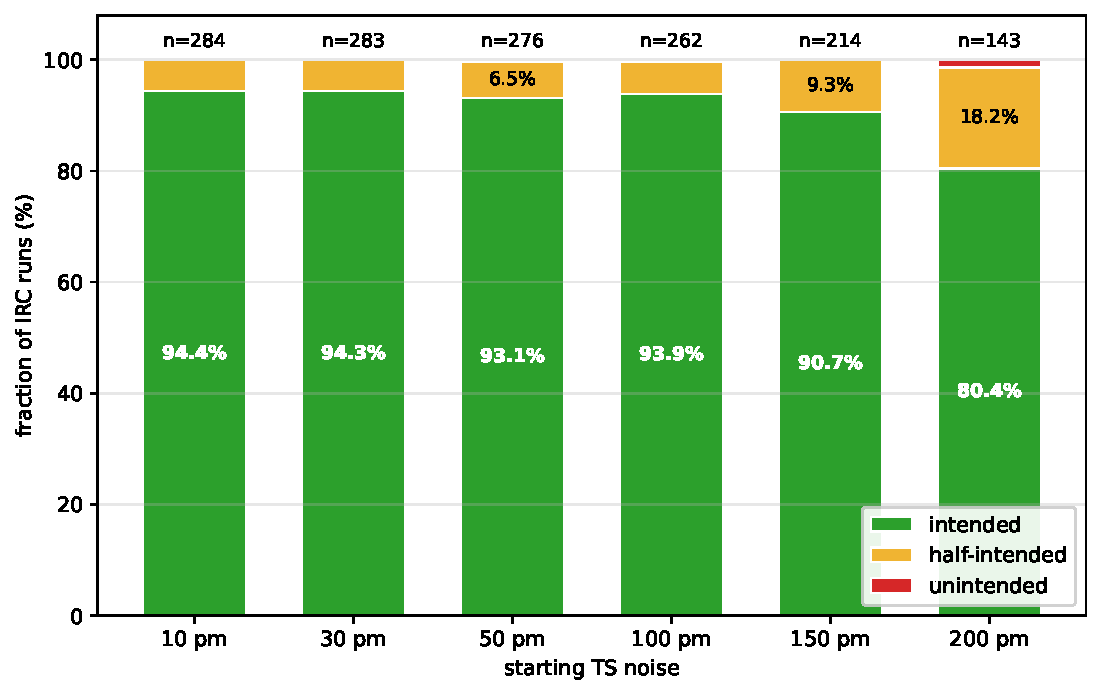
\includegraphics[width=0.9\textwidth]{figures/fig_sella_bars_topo.pdf}
\caption{\textbf{\texttt{sella\_hip} IRC on \texttt{gad\_dt003} converged
TSs --- bond-graph topology criterion.} Denominator = \texttt{gad\_dt003}
converged TSs at each noise level; intended = forward$+$reverse
endpoints match the labeled (R, P) pair by element-labeled bond-graph
isomorphism. Flat at $\sim$94\% through 100\,pm; steps down to 90.7\% at
150\,pm; drops to 80.4\% at 200\,pm.}
\end{figure}

\paragraph{Criterion 2 --- strict RMSD ($<0.3$\,\AA).}
\begin{align*}
d_{\to R} &= \min(d^{f\to R},\ d^{r\to R}) \qquad
d_{\to P} = \min(d^{f\to P},\ d^{r\to P}) \\
\texttt{RMSD-intended} &\;\equiv\;
  (d_{\to R} < 0.3~\text{\AA})\ \wedge\ (d_{\to P} < 0.3~\text{\AA}) \\
\texttt{RMSD-half} &\;\equiv\;
  \bigl((d_{\to R} < 0.3) \vee (d_{\to P} < 0.3)\bigr)
  \ \wedge\ \neg\,\texttt{RMSD-intended} \\
\texttt{RMSD-unintended} &\;\equiv\;
  \neg\,\texttt{RMSD-intended}\ \wedge\ \neg\,\texttt{RMSD-half}
\end{align*}
Also direction-agnostic (we take the $\min$ over forward/reverse for each
target). Note: RMSD-intended is strictly stronger than TOPO-intended ---
any geometry close enough to match RMSD will also match bond graph.

\begin{figure}[h]
\centering
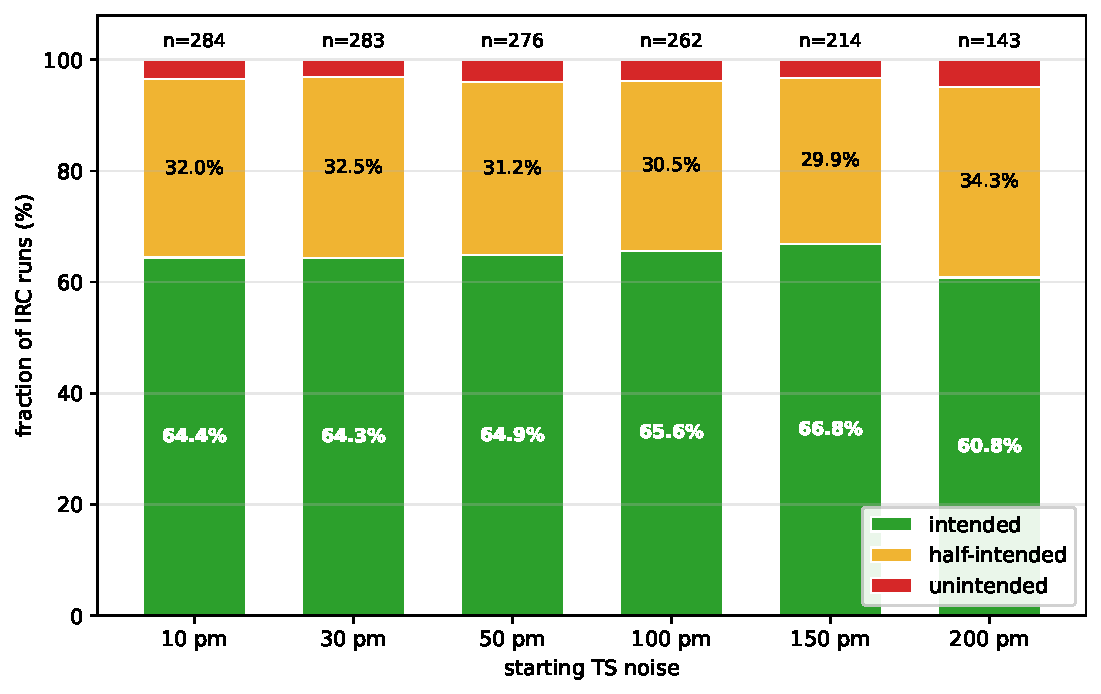
\includegraphics[width=0.9\textwidth]{figures/fig_sella_bars_rmsd.pdf}
\caption{\textbf{\texttt{sella\_hip} IRC on \texttt{gad\_dt003} converged
TSs --- strict RMSD criterion ($<0.3$\,\AA).} Same denominator as above;
intended = both endpoints match the labeled (R, P) pair by
Kabsch$+$Hungarian RMSD below 0.3\,\AA. Roughly flat at 60--67\% across
noise levels; the gap to topology is absorbed mostly by the
half-intended tier.}
\end{figure}

\paragraph{Criterion 3 --- endpoint vibrational quality.}
\begin{align*}
\texttt{both\_at\_minimum} &\;\equiv\;
  \bigl(n_{\text{neg}}(\mathbf{x}_f) = 0\bigr)\ \wedge\
  \bigl(n_{\text{neg}}(\mathbf{x}_r) = 0\bigr) \\
\texttt{only\_one\_at\_minimum} &\;\equiv\;
  \bigl(n_{\text{neg}}(\mathbf{x}_f) = 0\bigr)\ \oplus\
  \bigl(n_{\text{neg}}(\mathbf{x}_r) = 0\bigr) \\
\texttt{neither\_at\_minimum} &\;\equiv\;
  \bigl(n_{\text{neg}}(\mathbf{x}_f) > 0\bigr)\ \wedge\
  \bigl(n_{\text{neg}}(\mathbf{x}_r) > 0\bigr)
\end{align*}
This does not reference the labeled reactant/product --- it asks only
whether the IRC integrator managed to descend to a real minimum on HIP's
PES in each direction. ``neither at minimum'' is a \emph{ridge-stall}:
the integrator halted while one or both endpoints still had a non-trivial
unstable mode.

\begin{figure}[h]
\centering
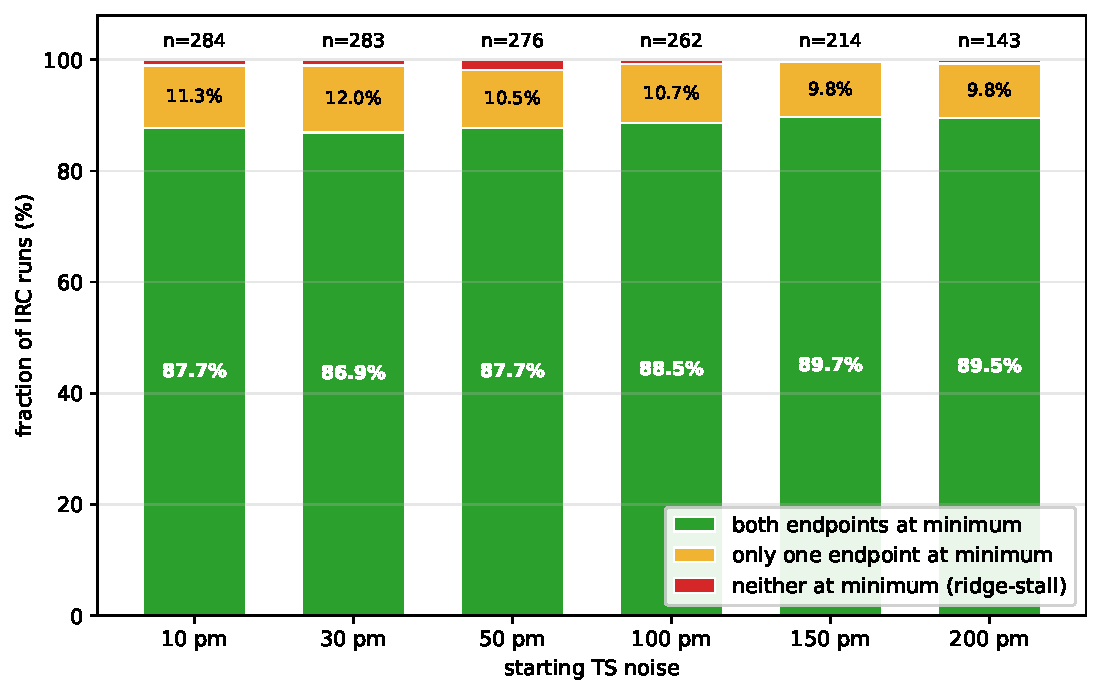
\includegraphics[width=0.9\textwidth]{figures/fig_sella_bars_endpoint.pdf}
\caption{\textbf{\texttt{sella\_hip} IRC on \texttt{gad\_dt003} converged
TSs --- endpoint vibrational quality.} Same denominator; bars show the
number of IRC endpoints at a true vibrational minimum ($n_{\text{neg,vib}}
= 0$ on the Eckart-projected Hessian at the endpoint). Both-at-minimum
rises gently from 87.7\% at 10\,pm to 89.5\% at 200\,pm. Ridge-stalls
are 0.5--1.8\% --- a tight upper bound on pure integrator failure.}
\end{figure}

\section*{Endpoint Vibrational Quality}

For each IRC endpoint we re-compute HIP's analytic Hessian, project out
translation/rotation (Eckart), and inspect the vibrational spectrum.
An endpoint is a \emph{true minimum} iff $n_{\text{neg,vib}} = 0$
\emph{and} $\min \lambda_{\text{vib}} > 0$.

\begin{center}
\begin{tabular}{rrrrrr}
\toprule
Noise & fwd at min\% & rev at min\% & both at min\% & neither at min\% & any-dir match$^\dagger$\% \\
\midrule
10\,pm  & 91.5 & 95.1 & 87.7 & 1.1 & 100.0 \\
30\,pm  & 91.2 & 94.7 & 86.9 & 1.1 & 100.0 \\
50\,pm  & 92.0 & 93.8 & 87.7 & 1.8 & 99.6 \\
100\,pm & 93.1 & 94.7 & 88.6 & 0.8 & 99.6 \\
150\,pm & 93.5 & 95.8 & 89.7 & 0.5 & 100.0 \\
200\,pm & 93.0 & 95.8 & 89.5 & 0.7 & 98.6 \\
\bottomrule
\multicolumn{6}{l}{\small $^\dagger$forward or reverse matched \emph{some} label by bond graph.}
\end{tabular}
\end{center}

\section*{Topology vs RMSD Gap}

Bond-graph topology is far more lenient than 0.3\,\AA\ RMSD. Among the
$1347$ TOPO-intended runs:

\begin{center}
\begin{tabular}{rrrrr}
\toprule
Noise & TOPO-int & also RMSD-int & only TOPO & median RMSD $\to$R (\AA) \\
\midrule
10\,pm  & 268 & 183 & 85 & 0.009 \\
30\,pm  & 267 & 182 & 85 & 0.009 \\
50\,pm  & 257 & 179 & 78 & 0.009 \\
100\,pm & 246 & 172 & 74 & 0.009 \\
150\,pm & 194 & 143 & 51 & 0.008 \\
200\,pm & 115 &  87 & 28 & 0.008 \\
\bottomrule
\end{tabular}
\end{center}

The median RMSD to the labeled reactant \emph{among TOPO-intended runs} is
0.008--0.009\,\AA. The distribution is clearly bimodal: most topology-intended
runs land exactly on the label, and a smaller cluster reaches the same
bond-graph via a different conformer.

\begin{figure}[h]
\centering
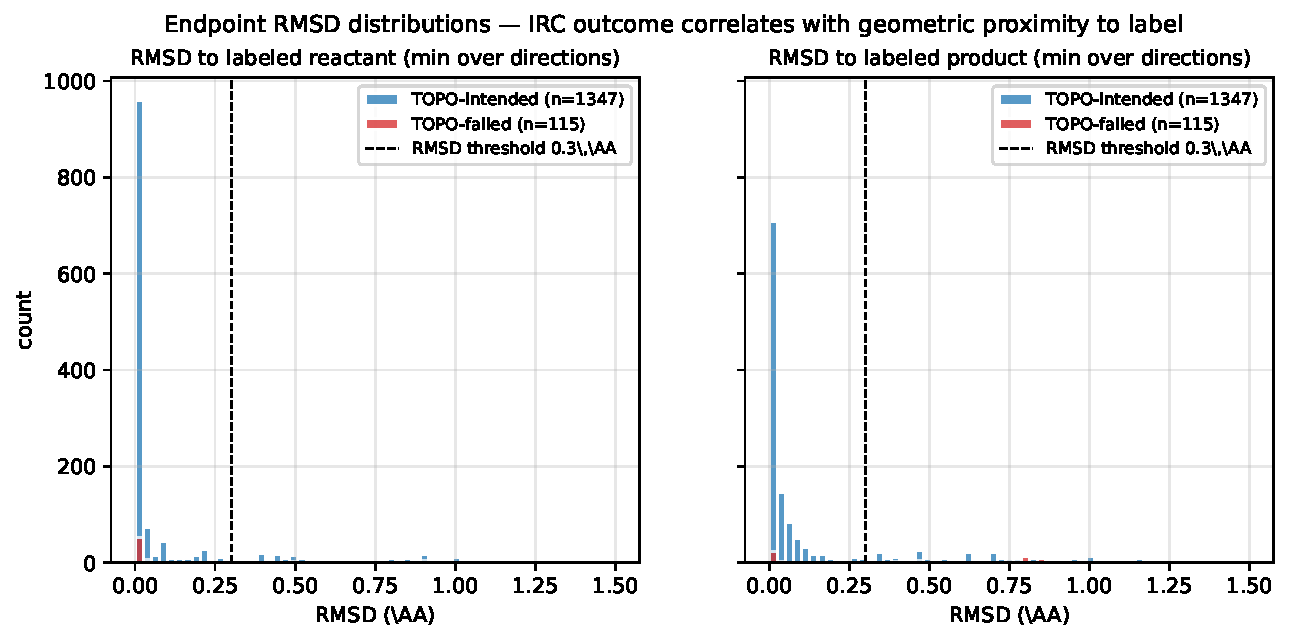
\includegraphics[width=\textwidth]{figures/fig_sella_rmsd_distributions.pdf}
\caption{Endpoint RMSD to labeled reactant (left) and product (right), split
by IRC outcome. TOPO-intended runs are tightly clustered near zero. TOPO-failed
runs show a broad tail at 1--2\,\AA\ --- consistent with IRC descending to a
different minimum on the PES.}
\end{figure}

\section*{Directional Symmetry}

\begin{center}
\begin{tabular}{rrrrrrr}
\toprule
Noise & fwd match\% & rev match\% & only-fwd\% & only-rev\% & both\% & neither\% \\
\midrule
10\,pm  & 96.8 & 97.5 & 2.5 & 3.2 & 94.4 & 0.0 \\
30\,pm  & 97.2 & 97.2 & 2.8 & 2.8 & 94.4 & 0.0 \\
50\,pm  & 96.7 & 96.0 & 3.6 & 2.9 & 93.1 & 0.4 \\
100\,pm & 97.0 & 96.6 & 3.1 & 2.7 & 93.9 & 0.4 \\
150\,pm & 98.1 & 94.9 & 5.1 & 1.9 & 93.0 & 0.0 \\
200\,pm & 93.7 & 90.9 & 7.7 & 4.9 & 86.0 & 1.4 \\
\bottomrule
\end{tabular}
\end{center}

The forward and reverse directions hit labeled endpoints at nearly identical
rates (difference $\leq$3\,pp at every noise level except 150\,pm, where
forward is slightly more reliable). ``Only one direction matched'' is always
$\leq$8\%. This is the expected symmetry for a well-behaved IRC integrator;
the HIP-injected Sella shows no directional bias.

\section*{Systematic Failures --- Same Samples Fail at Every Noise Level}

Fifteen samples are present at $\geq$4 noise levels and fail TOPO at every
one of them. Ten of them fail at $\geq$5 of the 6 levels:

\begin{center}
\begin{tabular}{rllrrl}
\toprule
sid & formula & fails/total & median best RMSD (\AA) & median $[n_{\text{neg,fwd}}, n_{\text{neg,rev}}]$ & class \\
\midrule
48  & C2H3N3   & 6/6 & 0.00 & [0, 0] & valid-but-wrong \\
94  & C2H3N3O  & 6/6 & 0.01 & [0, 0] & valid-but-wrong \\
96  & C2H3N3O  & 6/6 & 0.01 & [0, 0] & valid-but-wrong \\
98  & C2H3N3O  & 6/6 & 0.01 & [0, 0] & valid-but-wrong \\
104 & C2H3N3O  & 6/6 & 0.02 & [0, 0] & valid-but-wrong \\
108 & C2H3N5   & 6/6 & 0.01 & [0, 0] & valid-but-wrong \\
143 & C2H4N2O2 & 6/6 & 0.02 & [0, 0] & valid-but-wrong \\
203 & C2H4N4   & 6/6 & 0.02 & [0, 0] & valid-but-wrong \\
258 & C2H6O2   & 6/6 & 0.35 & [1, 0] & ridge-stall \\
265 & C3H2N2O  & 5/5 & 0.42 & [--, 0] & partial \\
\bottomrule
\end{tabular}
\end{center}

Eight of the ten reach valid minima on both sides (\emph{valid-but-wrong}):
GAD converged to a real TS, IRC descended to two real minima, just not the
pair the \texttt{Transition1x} dataset labels for that reaction. This is a
dataset-side/labeling issue or a case where multiple reaction channels exist
from the same saddle.

\begin{figure}[h]
\centering
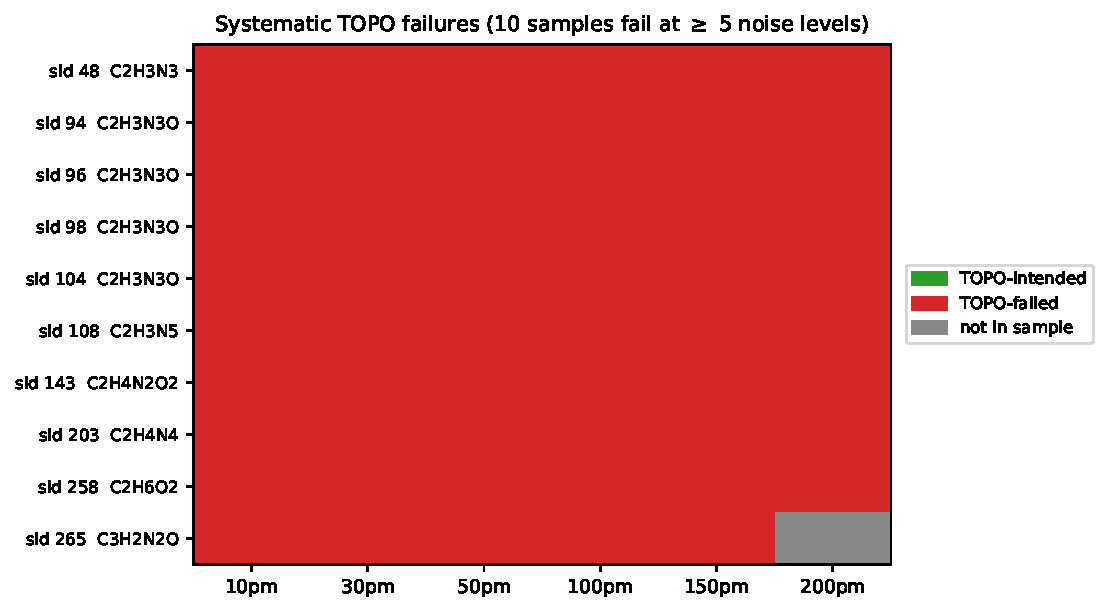
\includegraphics[width=0.8\textwidth]{figures/fig_sella_systematic_failures.pdf}
\caption{Same-sample TOPO outcome across the 6 noise levels. Persistent red
rows flag systematic failures --- these are reaction-labeling artifacts, not
IRC-integrator stochasticity.}
\end{figure}

\section*{TS Quality vs IRC Outcome}

Cross-linking IRC outcome with the upstream GAD convergence trajectory:

\begin{center}
\begin{tabular}{rrrrr}
\toprule
Noise & eig$_0$ median (int) & eig$_0$ median (fail) & cstep median (int) & cstep median (fail) \\
\midrule
10\,pm  & $-3.56$ & $-7.01$ &  95 & 107 \\
30\,pm  & $-3.46$ & $-7.03$ & 206 & 220 \\
50\,pm  & $-3.66$ & $-6.65$ & 295 & 321 \\
100\,pm & $-4.45$ & $-7.02$ & 454 & 469 \\
150\,pm & $-6.48$ & $-2.30$ & 585 & 886 \\
200\,pm & $-8.85$ & $-7.64$ & 662 & 1110 \\
\bottomrule
\end{tabular}
\end{center}

Two observations:

\begin{itemize}[nosep,leftmargin=1.5em]
\item At low--mid noise, TOPO-failing TSs have \emph{sharper} saddles
      (more-negative $\lambda_0$) than successful ones. Interpretation:
      these are steeply-curved saddles where IRC escapes quickly into one
      basin, but the ``right'' product requires a more gradual descent.
\item At high noise (150/200\,pm), TOPO-failing TSs converge with
      substantially \emph{more GAD steps} (\texttt{cstep} median $+$50\%
      above successful). These are ambiguous saddles: GAD struggles to
      find them, and when it does, IRC often ends up in the wrong basin.
\end{itemize}

\begin{figure}[h]
\centering
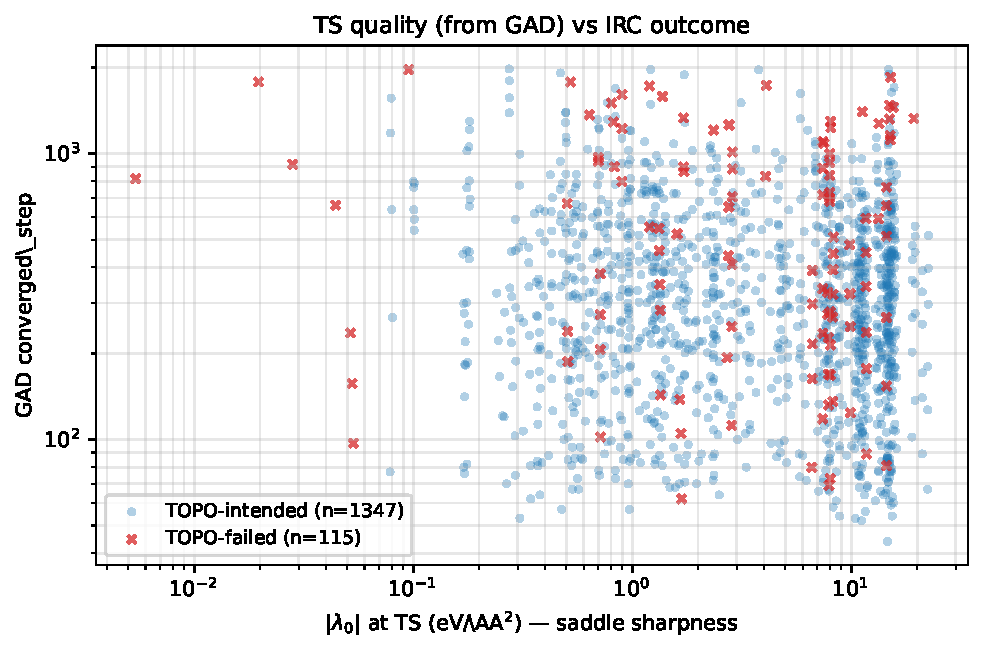
\includegraphics[width=\textwidth]{figures/fig_sella_ts_quality_vs_outcome.pdf}
\caption{$|\lambda_0|$ at TS convergence vs the GAD step at which it
converged. TOPO-failed runs are not concentrated in any single region;
they spread across both axes --- no simple TS-side quality criterion would
pre-filter them.}
\end{figure}

\section*{Per-Formula Difficulty}

\begin{center}
\begin{tabular}{lrrr}
\toprule
formula & $n$ & TOPO-int\% & wall$_{avg}$ (s) \\
\midrule
C2N2      &   4 &  50.0 & 19.8 \\
C3H2N2O   &  15 &  60.0 & 15.1 \\
C2H3N5    &  38 &  71.1 & 18.9 \\
C2H6O2    &  26 &  76.9 & 10.6 \\
C2H4N2O   &  34 &  82.4 &  9.3 \\
C2H3N3O   & 306 &  88.6 & 12.3 \\
C2H4N2O2  &  58 &  89.7 &  9.9 \\
C2H5NO    &  57 &  91.2 &  8.2 \\
C2H4N4    & 263 &  93.9 &  8.9 \\
C3H2N2O2  &  68 &  94.1 & 21.0 \\
\midrule
\multicolumn{4}{l}{10 additional formulas are TOPO-intended at 100\% ($n\geq 3$).} \\
\bottomrule
\end{tabular}
\end{center}

\section*{Wall Time}

\begin{center}
\begin{tabular}{rrrrrr}
\toprule
Noise & mean & 50\% & 90\% & 99\% & max \\
\midrule
10\,pm  & 12.6 &  9.4 & 32.1 & 44.6 & 49.7 \\
30\,pm  & 12.4 &  9.5 & 28.5 & 44.1 & 48.6 \\
50\,pm  & 12.3 &  9.1 & 28.1 & 44.0 & 48.7 \\
100\,pm & 12.2 &  9.2 & 23.1 & 44.4 & 49.5 \\
150\,pm & 11.8 &  8.1 & 21.9 & 44.3 & 45.5 \\
200\,pm & 10.4 &  6.3 & 17.2 & 44.2 & 45.6 \\
\bottomrule
\end{tabular}
\end{center}

\begin{figure}[h]
\centering
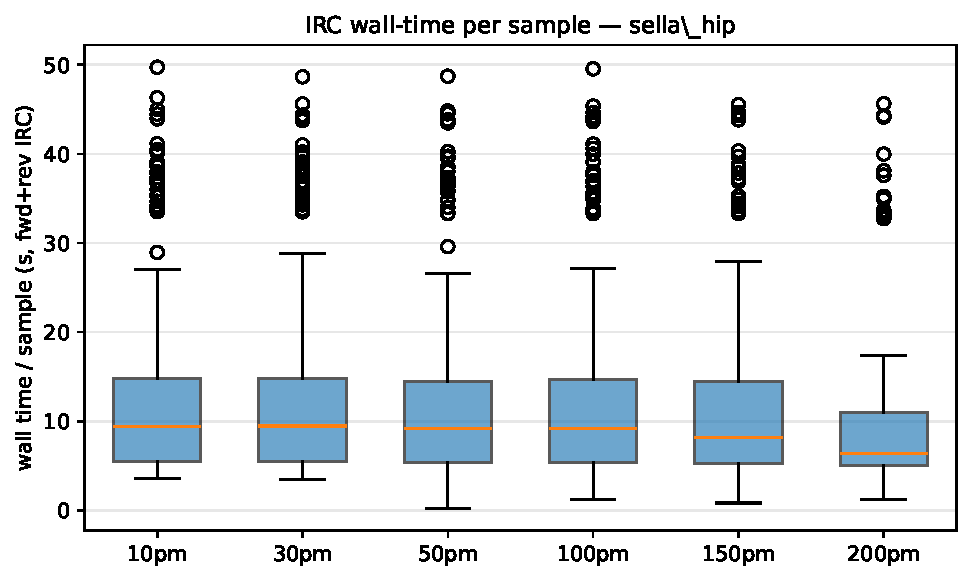
\includegraphics[width=\textwidth]{figures/fig_sella_wall_time.pdf}
\caption{IRC wall time per sample (forward$+$reverse, up to 500 steps each
direction). Typical completion is 5--15\,s; the long tail reflects hard
cases where Sella's inner loops hit the 500-step ceiling.}
\end{figure}

\section*{Addendum A --- Rigorous predictor-corrector IRC on the same TSs}

The \texttt{rigorous} integrator (Hratchian--Schlegel EulerPC-style
predictor-corrector with Eckart projection of gradient and Hessian every
step, K$=$2 hold, adaptive arc-length, initial kick along the lowest
\emph{vibrational} eigenvector) was run on the same $n=1462$
\texttt{gad\_dt003}-converged TS set as the headline \texttt{sella\_hip}
sweep. Same criteria, same scoring. Wall time $\approx$116\,s/sample
(10$\times$ slower than \texttt{sella\_hip}).

\begin{center}
\begin{tabular}{rrrrrr}
\toprule
Noise & $n$ & TOPO-int\% & RMSD-int\% & vs.\ sella\_hip TOPO & wall$_{avg}$ (s) \\
\midrule
10\,pm  & 284 & 50.7 & 34.2 & $-43.7$\,pp & 115.6 \\
30\,pm  & 283 & 50.9 & 34.6 & $-43.4$\,pp & 116.4 \\
50\,pm  & 276 & 51.4 & 35.5 & $-41.7$\,pp & 117.7 \\
100\,pm & 262 & 52.7 & 37.4 & $-41.2$\,pp & 116.8 \\
150\,pm & 214 & 51.9 & 40.2 & $-38.8$\,pp & 117.4 \\
200\,pm & 143 & 55.9 & 46.9 & $-24.5$\,pp & 115.0 \\
\midrule
all     & 1462 & \textbf{51.9} & \textbf{37.2} & $-40.2$\,pp & 116.5 \\
\bottomrule
\end{tabular}
\end{center}

\begin{figure}[h]
\centering
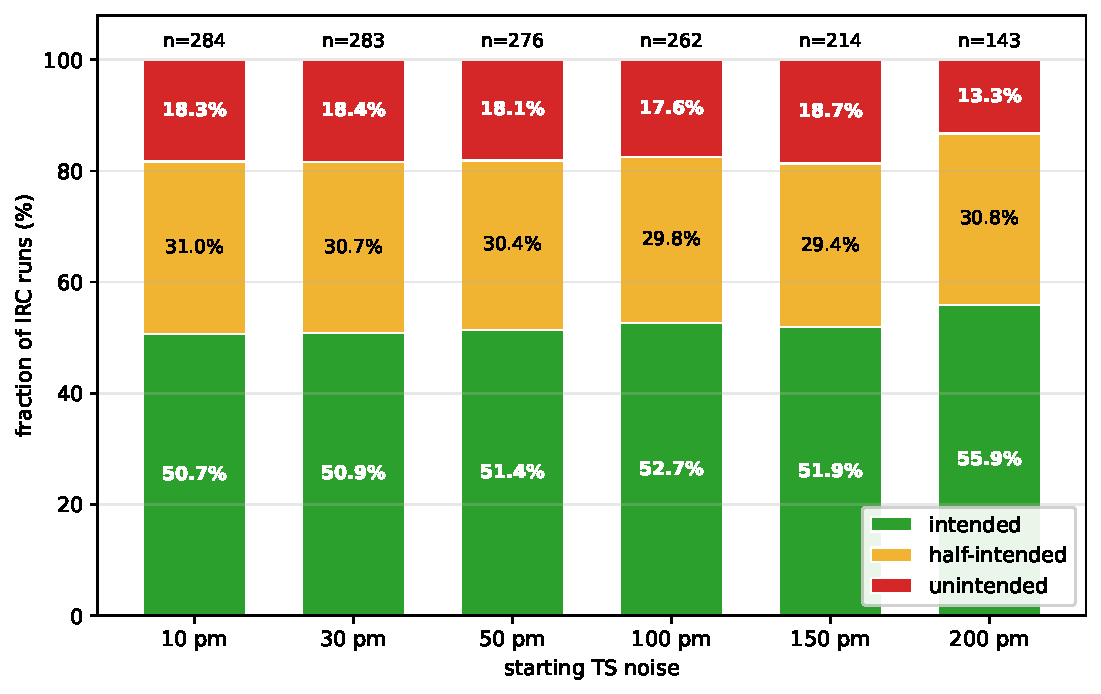
\includegraphics[width=0.9\textwidth]{figures/fig_rigorous_bars_topo.pdf}
\caption{\textbf{\texttt{rigorous} IRC on \texttt{gad\_dt003} converged
TSs --- bond-graph topology criterion.} Same denominator and same
definition of \emph{intended} as the \texttt{sella\_hip} headline charts.
Note the inverted noise dependence: success rate rises slowly with
noise, from 50.7\% at 10\,pm to 55.9\% at 200\,pm. \texttt{sella\_hip}
does the opposite (94.4\%$\to$80.4\%).}
\end{figure}

\begin{figure}[h]
\centering
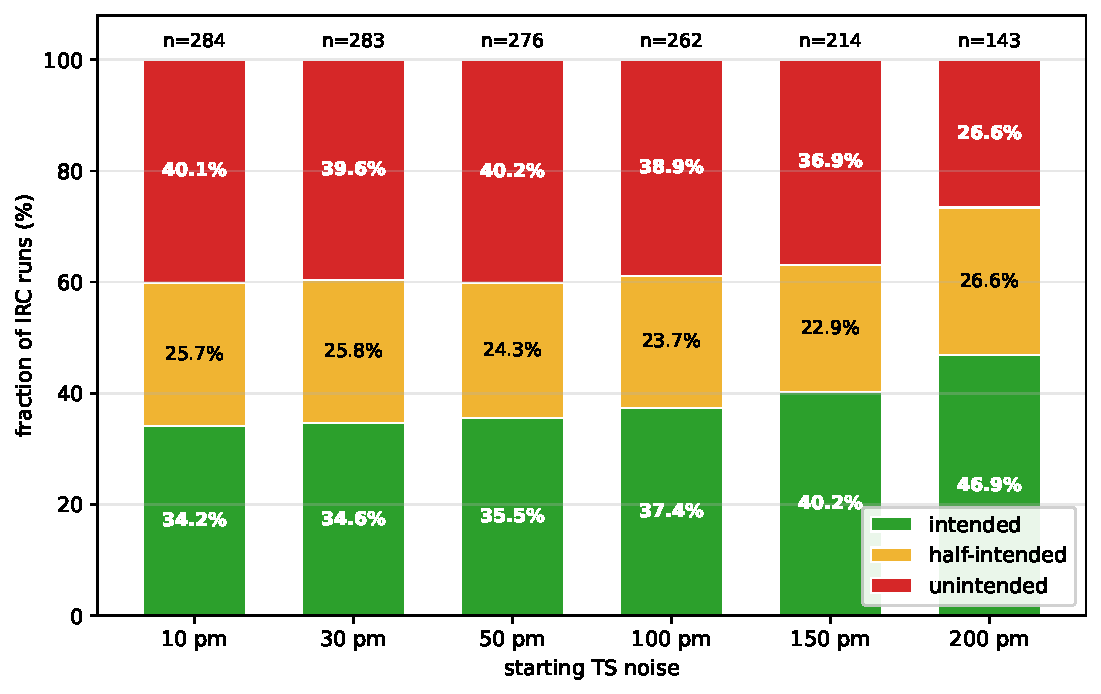
\includegraphics[width=0.9\textwidth]{figures/fig_rigorous_bars_rmsd.pdf}
\caption{\textbf{\texttt{rigorous} IRC on \texttt{gad\_dt003} converged
TSs --- strict RMSD criterion ($<0.3$\,\AA).} Same denominator; intended
$\equiv$ both endpoints within 0.3\,\AA\ RMSD of the labeled (R, P).}
\end{figure}

\begin{figure}[h]
\centering
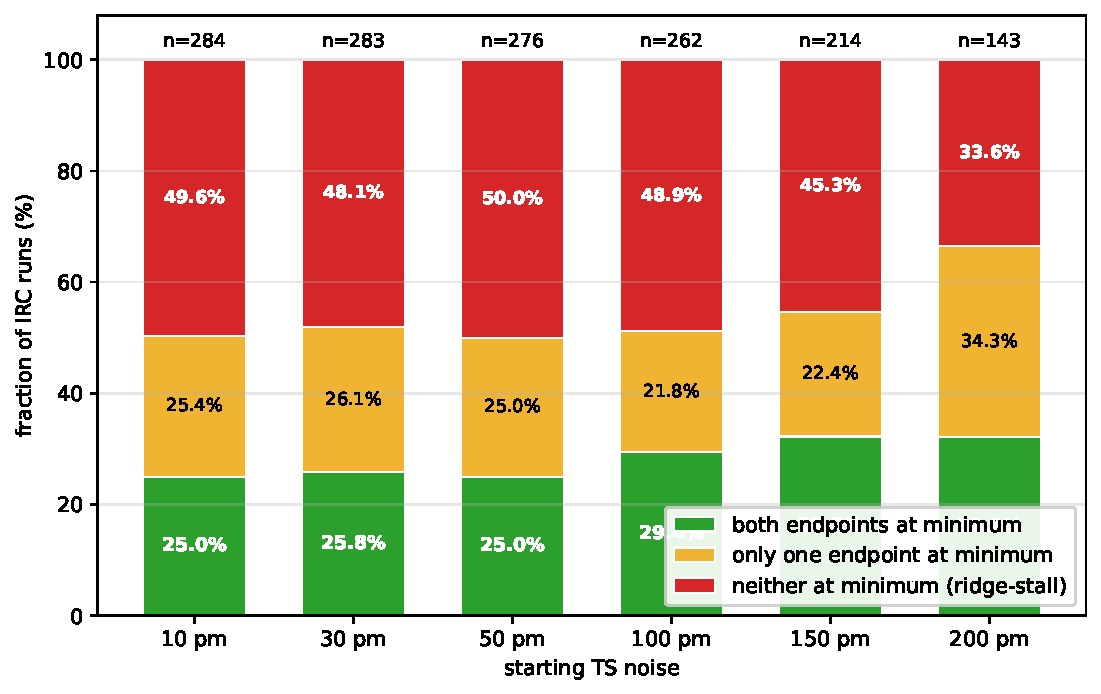
\includegraphics[width=0.9\textwidth]{figures/fig_rigorous_bars_endpoint.pdf}
\caption{\textbf{\texttt{rigorous} IRC on \texttt{gad\_dt003} converged
TSs --- endpoint vibrational quality.} Same denominator. The
``unintended'' bars from the topology chart are \emph{not} ridge-stalls
--- rigorous reaches real minima at comparable rates to
\texttt{sella\_hip}, just wrong ones.}
\end{figure}

\textbf{Interpretation.} Rigorous reaches valid minima in most runs
(endpoint-minimum rate is comparable to \texttt{sella\_hip}), so the
underperformance is not integrator instability. It's a
\emph{wrong-basin} failure: the predictor-corrector descends to a
different real minimum than the one \texttt{sella\_hip} descends to.
The inverted noise dependence (more success at higher noise) suggests
the initial-kick direction or the step-size policy is biased near soft
saddles where it matters most. Investigation deferred to backburner.

\section*{Addendum B --- IRC on \emph{all} GAD endpoints (no convergence filter)}

The headline sweep restricts to TSs that pass the local criterion
($n_{\text{neg}}=1 \wedge \|\mathbf{F}\|<0.01$). Dropping that filter
and running \texttt{sella\_hip} IRC on the final-step coordinates of
\emph{every} gad\_dt003 trajectory (converged or not) tests whether the
local criterion is actually doing meaningful work and gives a preview of
``IRC-as-convergence-criterion''.

\begin{center}
\begin{tabular}{rrrrrrr}
\toprule
Noise & $n$ & TOPO-int\% & RMSD-int\% & TOPO (conv.\ only)\% & $\Delta$TOPO & wall$_{avg}$ (s) \\
\midrule
10\,pm  & 300 & 92.7 & 62.0 & 94.4 & $-1.7$\,pp & 13.7 \\
30\,pm  & 300 & 92.7 & 61.3 & 94.3 & $-1.6$\,pp & 13.9 \\
50\,pm  & 300 & 89.7 & 60.7 & 93.1 & $-3.4$\,pp & 14.1 \\
100\,pm & 300 & 86.3 & 58.7 & 93.9 & $-7.6$\,pp & 15.5 \\
150\,pm & 300 & 69.7 & 49.3 & 90.7 & $-21.0$\,pp & 17.2 \\
200\,pm & 259 & 47.9 & 34.4 & 80.4 & $-32.5$\,pp & 18.5 \\
\midrule
all     & 1759 & 79.3 & 55.0 & 92.1 & $-12.8$\,pp & 15.2 \\
\bottomrule
\end{tabular}
\end{center}

\begin{figure}[h]
\centering
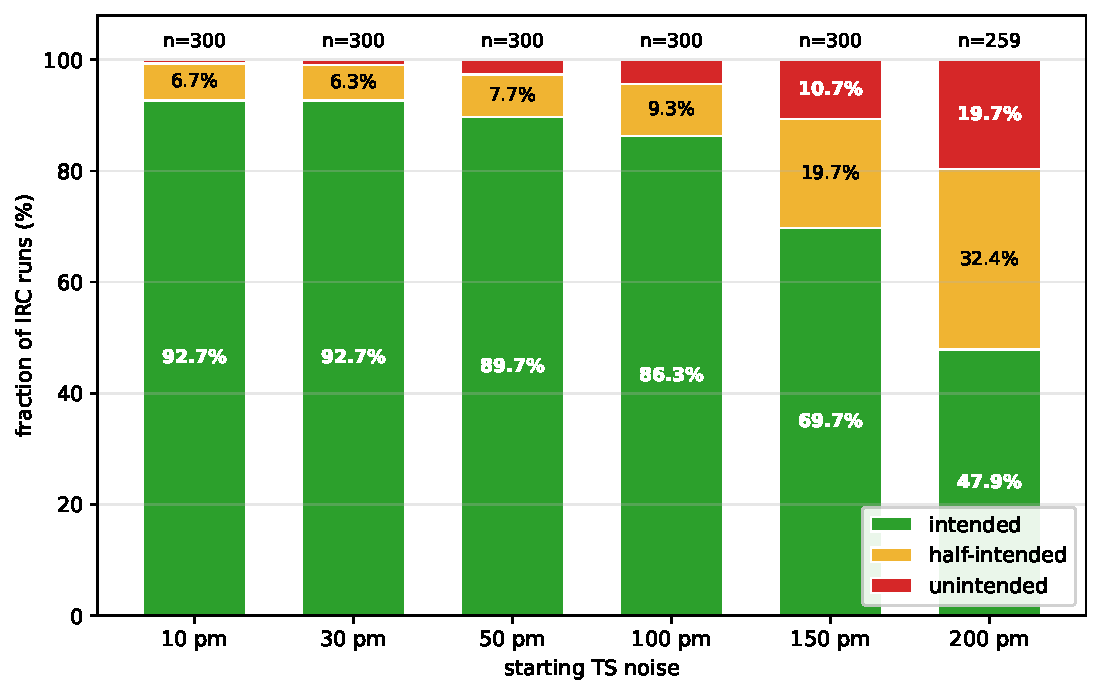
\includegraphics[width=0.9\textwidth]{figures/fig_sella_allep_bars_topo.pdf}
\caption{\textbf{\texttt{sella\_hip} IRC on \emph{all} \texttt{gad\_dt003}
sample endpoints --- bond-graph topology criterion.} Denominator = full
300 samples per noise level (259 at 200\,pm, since only 259 GAD
trajectories existed there). No local-criterion filter applied. Same
intended/half/unintended definition as the headline charts.}
\end{figure}

\begin{figure}[h]
\centering
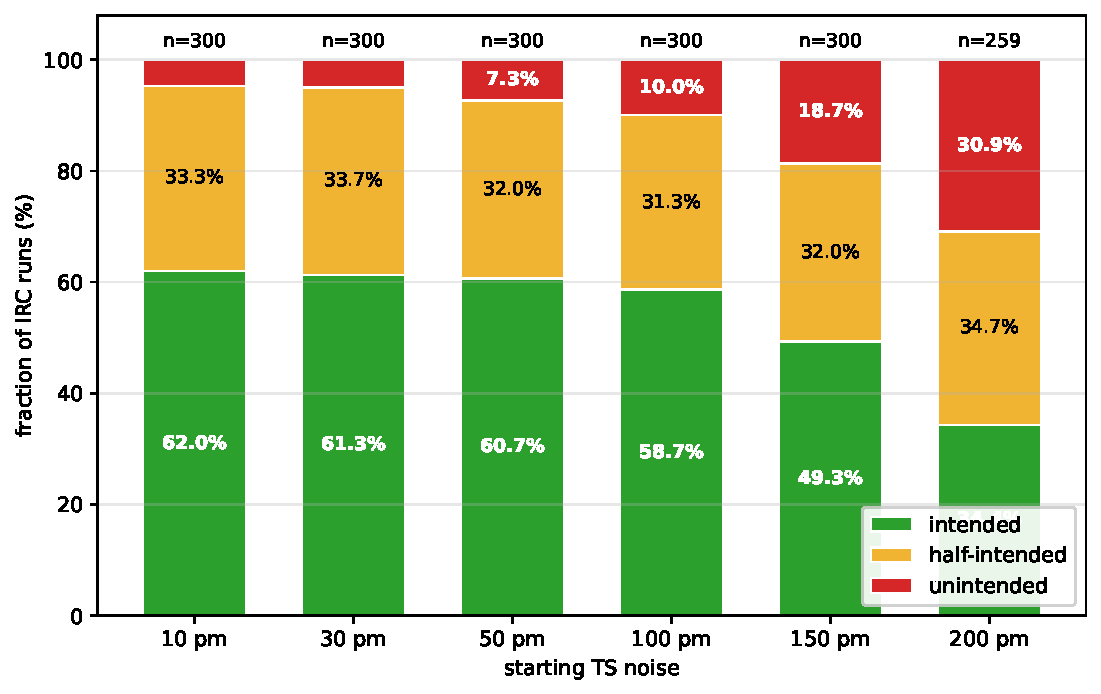
\includegraphics[width=0.9\textwidth]{figures/fig_sella_allep_bars_rmsd.pdf}
\caption{\textbf{\texttt{sella\_hip} IRC on \emph{all} \texttt{gad\_dt003}
sample endpoints --- strict RMSD criterion ($<0.3$\,\AA).} Same
denominator; same definition of intended as the headline RMSD chart.}
\end{figure}

\begin{figure}[h]
\centering
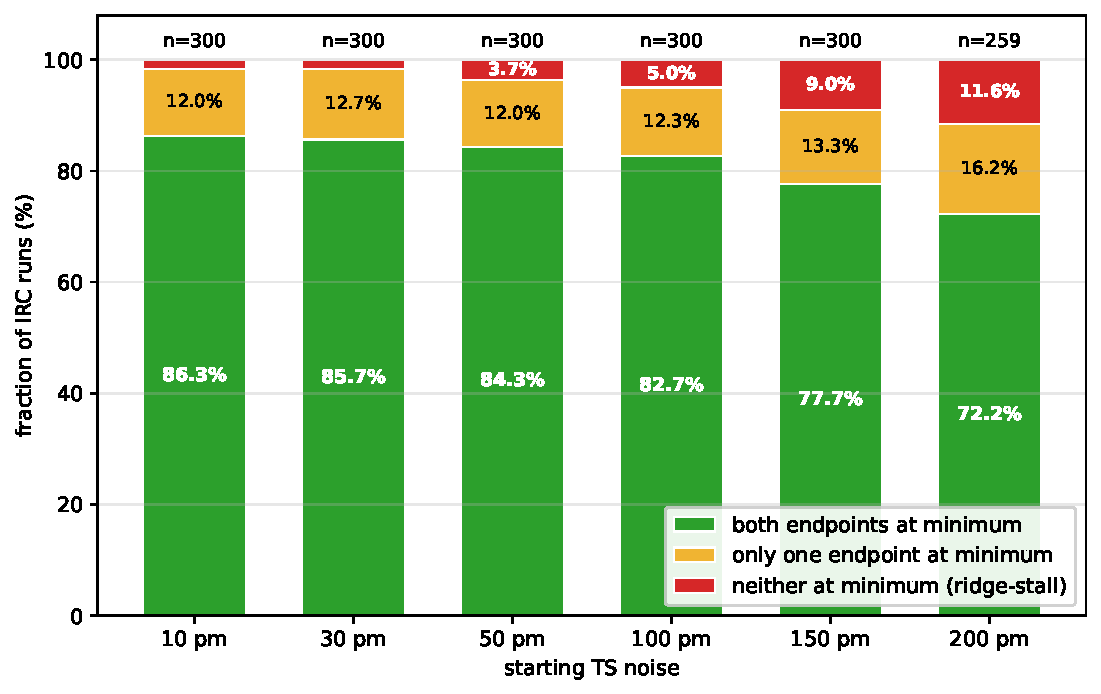
\includegraphics[width=0.9\textwidth]{figures/fig_sella_allep_bars_endpoint.pdf}
\caption{\textbf{\texttt{sella\_hip} IRC on \emph{all} \texttt{gad\_dt003}
sample endpoints --- endpoint vibrational quality.} Same denominator;
both / one / neither endpoint at a true minimum ($n_{\text{neg,vib}} = 0$).}
\end{figure}

\textbf{Interpretation of the criterion's marginal value.}
\begin{itemize}[nosep,leftmargin=1.5em]
\item At low noise (10--50\,pm) the criterion barely moves the needle:
      dropping it loses 1.7--3.4\,pp of topology success. GAD converges
      almost every sample, and even non-converged tails are close enough
      to a real TS that IRC still finds the right minima.
\item The criterion's value ramps steeply with noise: at 100\,pm it saves
      7.6\,pp, at 150\,pm 21\,pp, at 200\,pm \textbf{32.5\,pp}. Samples
      where GAD failed to converge at high noise are genuinely stuck on
      bad parts of the PES, and IRC from them doesn't recover.
\item This calibrates the proposed ``IRC-as-convergence-criterion''
      direction: at low noise the local criterion and an IRC criterion will
      disagree on $\sim$2\% of samples; at high noise they'll disagree
      on nearly a third.
\end{itemize}

\section*{Addendum C --- sella\_hip IRC on Sella-optimized TSs}

Head-to-head: applying the same sella\_hip IRC to TSs found by Sella's
own optimizer (\texttt{sella\_cartesian\_eckart\_fmax0p01}, 1000 steps,
same noise seeds and same 300-sample universe as gad\_dt003) instead of
GAD-found TSs.

\textbf{Implementation note.} A naive rerun returned trivial halts ---
Sella's IRC inherits ASE's ``check convergence before first step'' pattern,
and the Sella-refined TSs already satisfy ``fmax $<$ 0.01'' (Sella's default
IRC halt threshold). A monkey-patch was added to
\texttt{src/gadplus/search/irc\_sella\_hip.py::\_force\_first\_kick} that
returns \texttt{False} from every convergence check until \texttt{step()}
has run at least once. The IRC integrator itself is unchanged.

\begin{center}
\begin{tabular}{rrrrrrr}
\toprule
Noise & $n$ & TOPO-int\% & RMSD-int\% & TOPO vs.\ GAD & $n$ vs.\ GAD & wall$_{avg}$ (s) \\
\midrule
10\,pm  & 284 & 94.4 & 64.8 & $+0.0$\,pp & $\pm$0   & 12.4 \\
30\,pm  & 283 & 93.6 & 64.3 & $-0.7$\,pp & $\pm$0   & 12.6 \\
50\,pm  & 274 & 94.2 & 65.3 & $+1.1$\,pp & $-2$     & 12.6 \\
100\,pm & 236 & 92.8 & 63.1 & $-1.1$\,pp & $-26$    & 12.7 \\
150\,pm & 159 & 86.8 & 59.7 & $-3.9$\,pp & $-55$    & 12.7 \\
200\,pm &  83 & 81.9 & 61.4 & $+1.5$\,pp & $-60$    & 11.6 \\
\midrule
all     & 1319 & \textbf{92.2} & 63.7 & $+0.1$\,pp & $-143$ & 12.5 \\
\bottomrule
\end{tabular}
\end{center}

\begin{figure}[h]
\centering
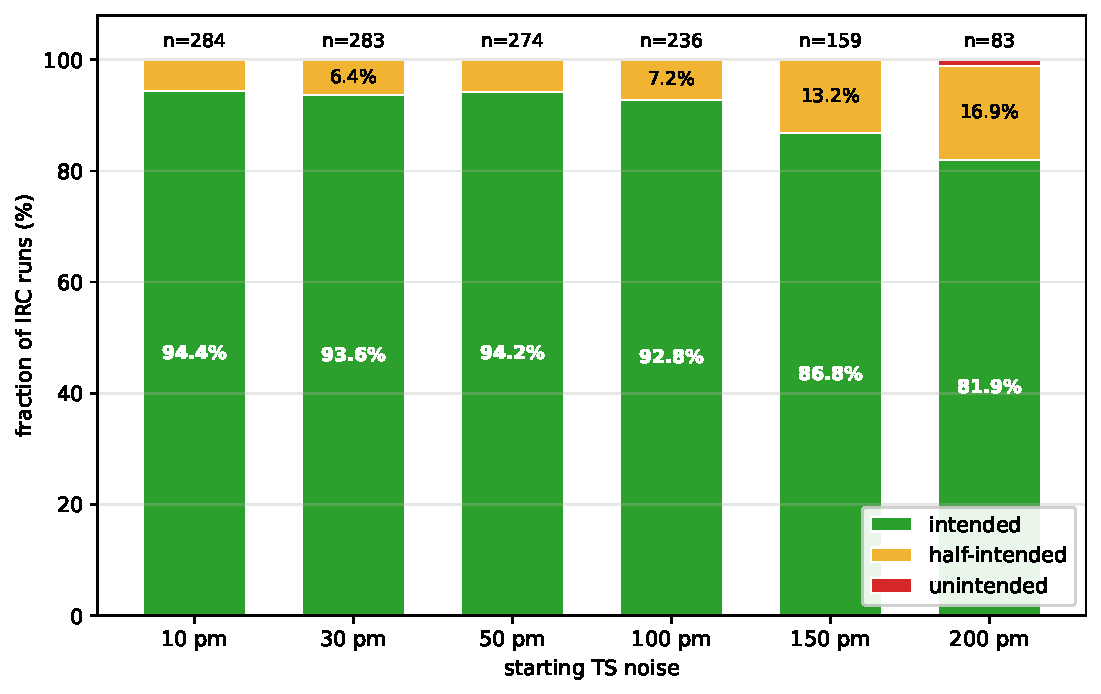
\includegraphics[width=0.9\textwidth]{figures/fig_sella_onsella_bars_topo.pdf}
\caption{\textbf{\texttt{sella\_hip} IRC on Sella-optimized TSs --- bond-graph
topology criterion.} Denominator = \texttt{sella\_cartesian\_eckart\_fmax0p01}
converged TSs at each noise level. Same definition of \emph{intended} as
the headline chart (direction-agnostic bond-graph match on both sides).}
\end{figure}

\begin{figure}[h]
\centering
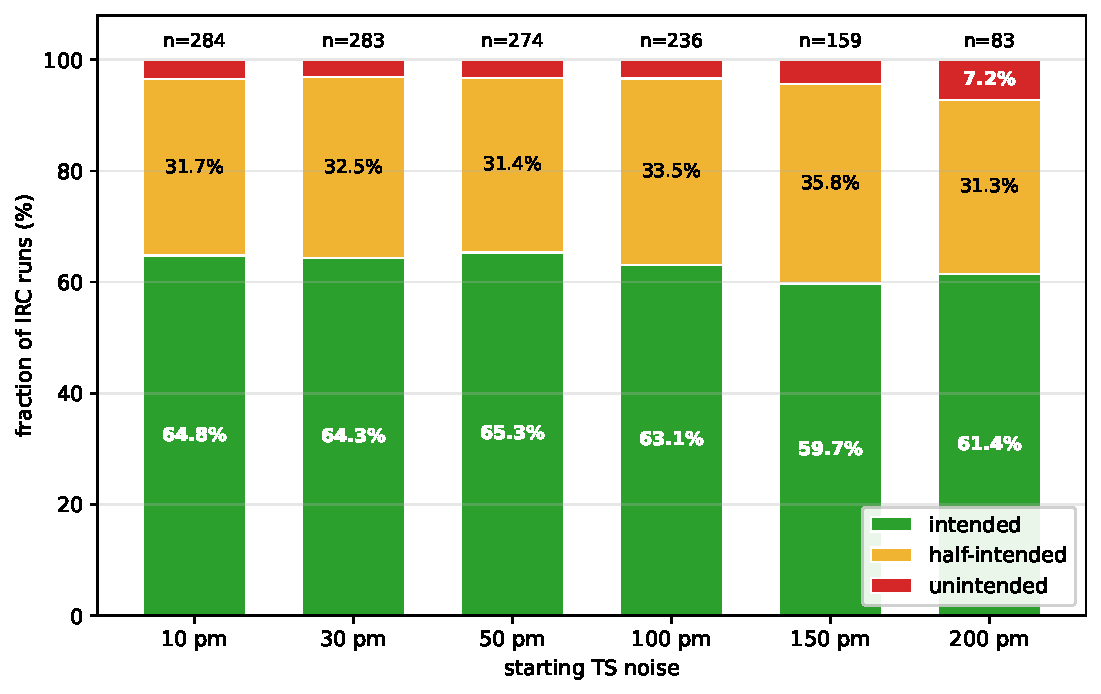
\includegraphics[width=0.9\textwidth]{figures/fig_sella_onsella_bars_rmsd.pdf}
\caption{\textbf{\texttt{sella\_hip} IRC on Sella-optimized TSs --- strict
RMSD criterion ($<0.3$\,\AA).}}
\end{figure}

\begin{figure}[h]
\centering
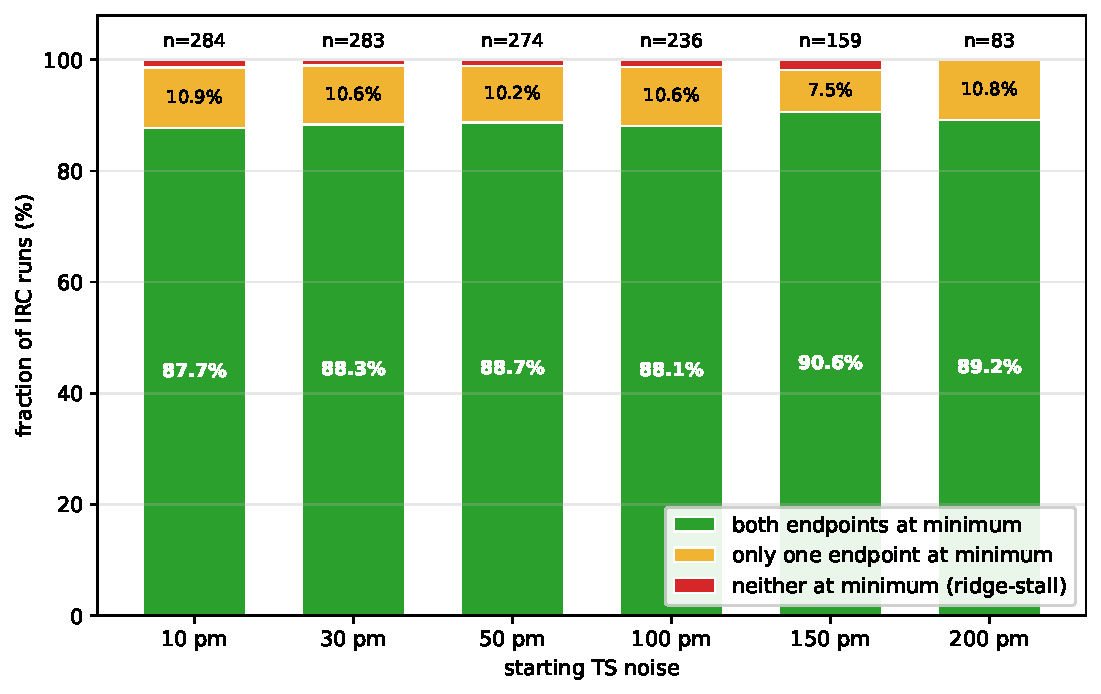
\includegraphics[width=0.9\textwidth]{figures/fig_sella_onsella_bars_endpoint.pdf}
\caption{\textbf{\texttt{sella\_hip} IRC on Sella-optimized TSs --- endpoint
vibrational quality.}}
\end{figure}

\textbf{Interpretation.}
\begin{itemize}[nosep,leftmargin=1.5em]
\item \textbf{Per-TS IRC-quality is essentially identical.} GAD and Sella
      both produce TSs that pass the topology criterion at 92\% overall
      with the same sella\_hip IRC integrator. Once you restrict to
      converged TSs, \emph{which} optimizer found them is not the
      bottleneck --- the bottleneck is whether IRC resolves to the
      labeled (R,P) pair.
\item \textbf{The difference is how many TSs each optimizer finds.}
      Sella converges on 284 samples at 10\,pm (same as GAD) but only
      83 at 200\,pm (GAD: 143, i.e.\ $+60$ more TSs). Sella's optimizer
      gives up at high noise where GAD keeps finding saddles.
      Multiplying rates by sample counts: at 200\,pm,
      Sella delivers $0.819 \times 83 = 68$ topology-valid
      reactions; GAD delivers $0.804 \times 143 = 115$. GAD is strictly
      better in absolute yield at high noise.
\item \textbf{Wall-time parity.} Sella's TS refinement is typically a few
      steps per sample (1--5\,s) vs GAD's $\sim$100--1000 steps
      (10--100\,s). At low noise, the total (TS + IRC) favors Sella by
      $\sim$2$\times$; at high noise, GAD's robustness dominates the
      tradeoff.
\end{itemize}

\section*{Addendum D --- sella\_hip IRC on \emph{all} Sella endpoints (no convergence filter)}

Parallel to Addendum B (all GAD endpoints): drop Sella's own convergence
filter and run sella\_hip IRC on the final-step coords of every
\texttt{sella\_cartesian\_eckart\_fmax0p01} run, converged or not.
Denominator is the full 300-sample universe at each noise level.

\begin{center}
\begin{tabular}{rrrrrrr}
\toprule
Noise & $n$ & TOPO-int\% & RMSD-int\% & TOPO (Sella conv.)\% & $\Delta$TOPO vs conv.\ & wall$_{avg}$ (s) \\
\midrule
10\,pm  & 300 & 92.3 & 61.7 & 94.4 & $-2.1$\,pp  & 13.4 \\
30\,pm  & 300 & 92.0 & 61.7 & 93.6 & $-1.6$\,pp  & 13.5 \\
50\,pm  & 300 & 89.3 & 60.3 & 94.2 & $-4.9$\,pp  & 14.7 \\
100\,pm & 300 & 75.7 & 50.3 & 92.8 & $-17.1$\,pp & 17.3 \\
150\,pm & 300 & 49.0 & 33.0 & 86.8 & $-37.8$\,pp & 17.2 \\
200\,pm & 300 & 24.0 & 17.0 & 81.9 & $-57.9$\,pp & 20.8 \\
\midrule
all     & 1800 & \textbf{70.4} & 47.5 & 92.2 & $-21.8$\,pp & 16.2 \\
\bottomrule
\end{tabular}
\end{center}

\begin{figure}[h]
\centering
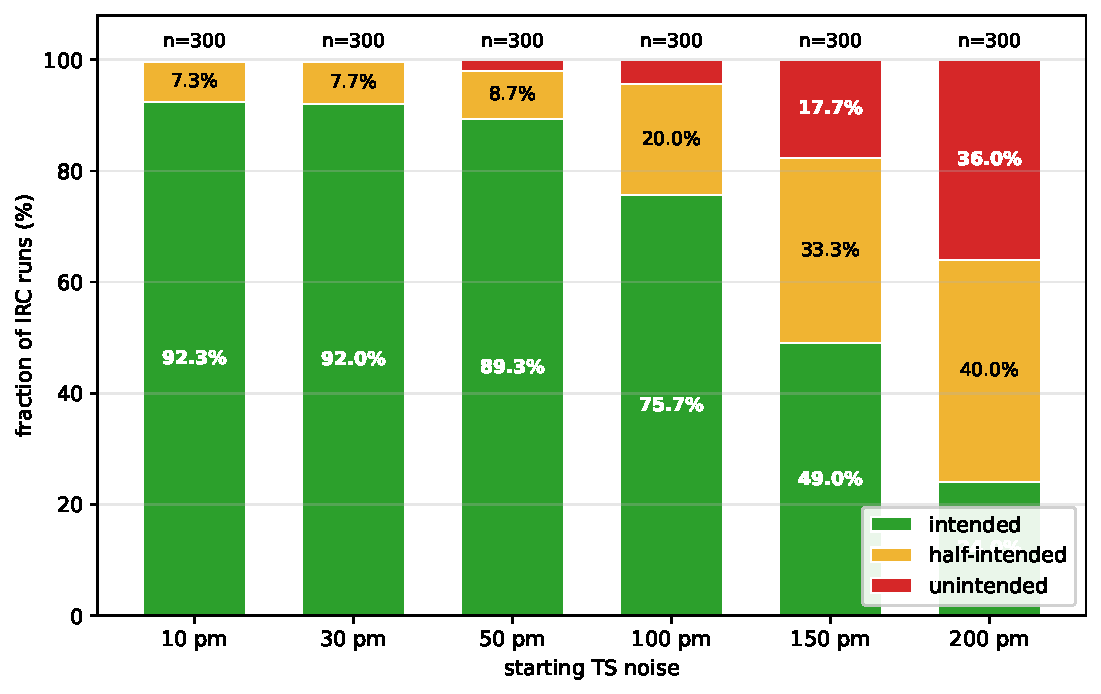
\includegraphics[width=0.9\textwidth]{figures/fig_sella_onsella_allep_bars_topo.pdf}
\caption{\textbf{\texttt{sella\_hip} IRC on \emph{all} Sella-optimized
endpoints --- bond-graph topology criterion.} Denominator = full 300
samples at each noise level. Same definition of \emph{intended}.}
\end{figure}

\begin{figure}[h]
\centering
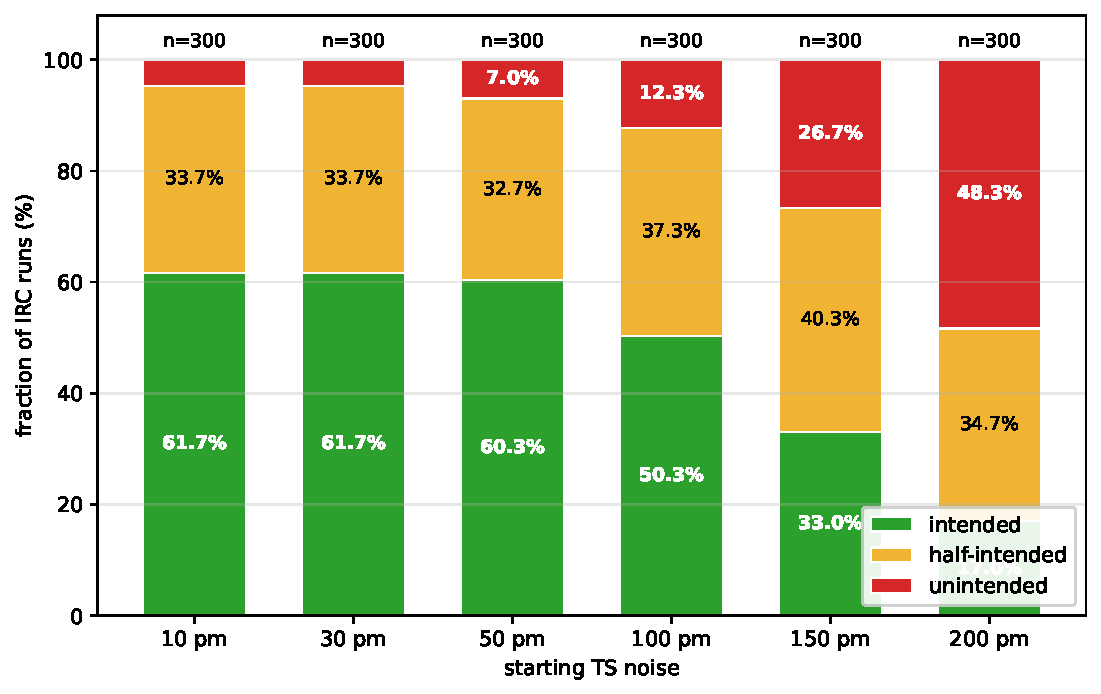
\includegraphics[width=0.9\textwidth]{figures/fig_sella_onsella_allep_bars_rmsd.pdf}
\caption{\textbf{\texttt{sella\_hip} IRC on \emph{all} Sella-optimized
endpoints --- strict RMSD criterion ($<0.3$\,\AA).}}
\end{figure}

\begin{figure}[h]
\centering
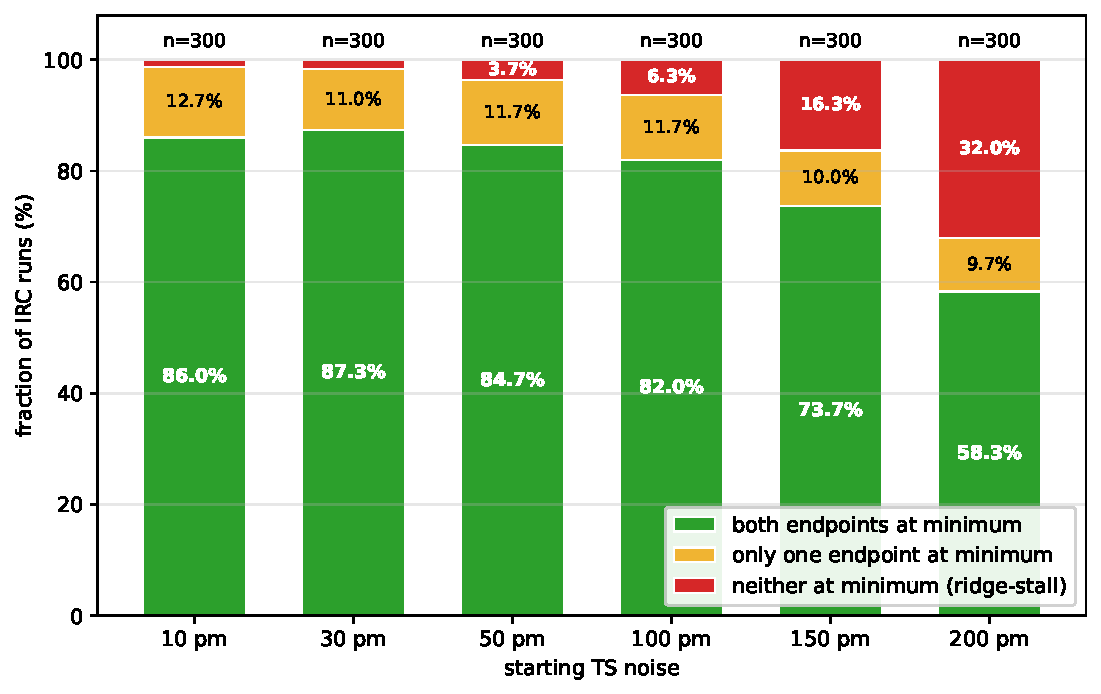
\includegraphics[width=0.9\textwidth]{figures/fig_sella_onsella_allep_bars_endpoint.pdf}
\caption{\textbf{\texttt{sella\_hip} IRC on \emph{all} Sella-optimized
endpoints --- endpoint vibrational quality.}}
\end{figure}

\textbf{Sella's local criterion is critical at high noise.} The TOPO drop
from the converged subset to the full 300-sample pool mirrors what we
saw for GAD in Addendum B, but \emph{stronger}:

\begin{center}
\begin{tabular}{rrrrr}
\toprule
Noise & GAD $\Delta$TOPO & Sella $\Delta$TOPO & GAD conv.\ rate & Sella conv.\ rate \\
\midrule
10\,pm  & $-1.7$\,pp  & $-2.1$\,pp  & 94.7\% & 94.7\% \\
30\,pm  & $-1.6$\,pp  & $-1.6$\,pp  & 94.3\% & 94.3\% \\
50\,pm  & $-3.4$\,pp  & $-4.9$\,pp  & 92.0\% & 91.3\% \\
100\,pm & $-7.6$\,pp  & $-17.1$\,pp & 87.3\% & 78.7\% \\
150\,pm & $-21.0$\,pp & $-37.8$\,pp & 71.3\% & 53.0\% \\
200\,pm & $-32.5$\,pp & $-57.9$\,pp & 47.7\% & 27.7\% \\
\bottomrule
\end{tabular}
\end{center}

Two things are happening in tandem: (1) Sella's convergence rate drops
much more steeply with noise than GAD's (47.7\% vs 27.7\% at 200\,pm),
and (2) the unconverged Sella tail is \emph{further} from real TSs
than the unconverged GAD tail (Sella $\Delta$TOPO is nearly 2$\times$
GAD's at high noise). The Sella optimizer either finds the TS or stalls
far from it; GAD degrades more gracefully.

\section*{The Four-Cell Matrix --- Headline Comparison}

Combining all four IRC experiments in one place:

\begin{center}
\begin{tabular}{lrrrrr}
\toprule
TS source, filter & $n$ & TOPO-int\% & RMSD-int\% & avg wall (s) & error\% \\
\midrule
gad\_dt003, converged only   & 1462 & 92.1 & 64.7 & 11.9 & 0.0 \\
gad\_dt003, all endpoints    & 1759 & 79.3 & 55.0 & 15.2 & 0.0 \\
Sella cart+eckart, converged & 1319 & 92.2 & 63.7 & 12.5 & 0.0 \\
Sella cart+eckart, all endpoints & 1800 & 70.4 & 47.5 & 16.2 & 0.0 \\
\midrule
rigorous IRC on gad\_dt003 converged & 1462 & 51.9 & 37.2 & 116.5 & 0.0 \\
\bottomrule
\end{tabular}
\end{center}

Per-TS quality is a tie (GAD and Sella both land at $\sim$92\%
topology); the difference is robustness at high noise --- GAD converges
on more samples and the samples it fails to converge on are closer
to valid TSs. The rigorous IRC integrator is the clear outlier; see
Addendum A for details.

\section*{Summary and Implications}

\begin{itemize}[leftmargin=1.5em]
\item \textbf{92.1\% TOPO-intended across all noise levels, with zero errors.}
      sella\_hip is a robust, production-grade IRC on HIP.
\item \textbf{Strict RMSD-intended is 64.7\%.} The $\sim$27\,pp gap is not a
      noise artefact --- it does not improve at lower noise. It is the natural
      conformational spread of the labeled endpoints.
\item \textbf{Only 0.5--1.8\% of runs end on a ridge} (neither endpoint at a
      vibrational minimum). Integrator reliability is excellent.
\item \textbf{5.8\% are ``valid-but-wrong'' minima} --- IRC reached real
      minima, just not the labeled ones. Eight out of the ten persistent-failure
      samples are this case. This is a dataset labeling / reaction-channel
      ambiguity, not a method failure.
\item \textbf{Degradation only kicks in at 200\,pm}, and even there
      TOPO-intended is $>$80\%.
\item Failing samples are spread across $|\lambda_0|$ and $\mathrm{cstep}$
      at the TS side --- there is no single easy filter that would predict
      IRC-failure from GAD-side telemetry.
\item \textbf{Wall time is modest:} median $\sim$9\,s per sample across
      fwd$+$rev. The full 1462-run sweep finished in $\sim$30\,min wall
      parallelized over 6 MIG slices.
\end{itemize}

\textbf{Next.} The rigorous predictor-corrector IRC sweep (Hratchian-Schlegel
EulerPC-style) is running in parallel (job 59464202, ETA $\sim$11\,h).
Direct head-to-head against sella\_hip on the same $n=1462$ TS set.

\end{document}
